%!TEX encoding = UTF-8 Unicode
%!TEX root = ../lect-week02.tex

%\Subsection{Samlingar och loopar}
\Subsection{Datastrukturer och kontrollstrukturer}


\begin{Slide}{Vad är en datastruktur?}\SlideFontSmall
\begin{itemize}
\item En \href{https://sv.wikipedia.org/wiki/Datastruktur}{datastruktur} är en struktur för organisering av data som...
\begin{itemize}\SlideFontTiny
\item kan innehålla \Alert{många} element,
\item kan refereras till med \Alert{ett} enda namn, och
\item ger möjlighet att komma åt de enskilda elementen.
\end{itemize}

\item En \Emph{samling} \Eng{collection} är en datastruktur som kan innehålla många element av \Alert{samma typ}.

\item Exempel på olika samlingar där elementen är organiserade på olika vis: \\ 
\vspace{0.5em}
\begin{tabular}{l c}
\Emph{Lista} & 
\includegraphics[width=5cm]{../img/list.pdf} \\
\Emph{Träd}  & 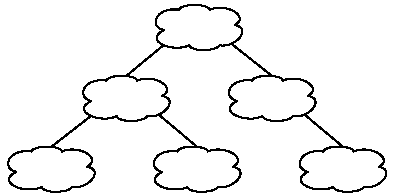
\includegraphics[width=2.2cm]{../img/tree.pdf} \\
\Emph{Graf}  & 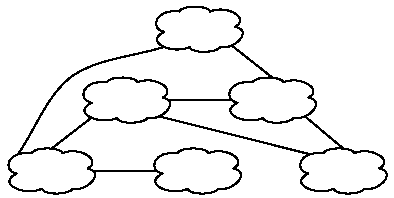
\includegraphics[width=2.2cm]{../img/graph.pdf} \\
\end{tabular}
\end{itemize}
{
\SlideFontTiny \vspace{1em }\hskip2em
Mer om listor \& träd \href{http://cs.lth.se/edaa01vt}{fördjupningskursen}. 
Mer om träd, grafer i \href{http://cs.lth.se/edaa40}{Diskreta strukturer.}
}

\end{Slide} 


\begin{Slide}{Vad är en vektor?}\SlideFontSmall
En \Emph{vektor}\footnote{Vektor kallas ibland på svenska även \href{https://sv.wikipedia.org/wiki/F\%C3\%A4lt_\%28datastruktur\%29}{fält}, men det skapar stor förvirring eftersom det engelska ordet \emph{field} ofta används för \emph{attribut} (förklaras senare).} 
\Eng{vector, \href{https://en.wikipedia.org/wiki/Array_data_structure}{array}} är en \Emph{samling} som är \Alert{snabb} att \Emph{indexera} i. 
Åtkomst av element sker med \code{apply(platsnummer)}: 

\begin{REPL}
scala> val heltal = Vector(42, 13, -1, 0 , 1)
heltal: scala.collection.immutable.Vector[Int] = Vector(42, 13, -1, 0, 1)

scala> heltal.apply(0)
res0: Int = 42

scala> heltal(1)    // man kan skippa .apply
res1: Int = 13

scala> heltal(5)
java.lang.IndexOutOfBoundsException: 5
  at scala.collection.immutable.Vector.checkRangeConvert(Vector.scala:132)
\end{REPL}
Utelämnar du \code{.apply} så gör kompilatorn anrop av \code{apply} ändå om det går.
\end{Slide}

\begin{Slide}{En konceptuell bild av en vektor}

\begin{REPLnonum}
scala> val heltal = Vector(42, 13, -1, 0 , 1)
\end{REPLnonum}

\begin{tikzpicture}[font=\ttfamily]
\matrix [matrix of nodes, row sep=0, column 2/.style={nodes={rectangle,draw,minimum width=3em}}] (var) at (0cm, 2.8cm)
{
heltal   &  \makebox(16,12){ }\\
};
\matrix [matrix of nodes, draw=black,row sep=0, column 2/.style={nodes={rectangle,draw,minimum width=4em}}] (vec) at (4cm, 1cm)
{
\textit{plats} &  \\
0   &  \makebox(16,12){42}\\
1   &  \makebox(16,12){13}\\
2   &  \makebox(16,12){-1}\\
3   &  \makebox(16,12){0}\\
4   &  \makebox(16,12){1}\\
};
\filldraw[black] (0.7cm,2.8cm) circle (3pt) node[] (ref) {};
 \draw [arrow] (ref) -- (vec);
\end{tikzpicture}

\vspace{1em} Elementen ligger på rad någonstans i minnet.
\end{Slide}



\begin{Slide}{En samling strängar}

\begin{itemize}
\item En vektor kan lagra många värden av samma typ. 
\item Elementen kan vara till exempel heltal eller strängar. 
\item Eller faktiskt vad som helst. 
\end{itemize}

\begin{REPL}
scala> val grönsaker = Vector("gurka","tomat","paprika","selleri")
grönsaker: scala.collection.immutable.Vector[String] = Vector(gurka, tomat, paprika, selleri)

scala> val g = grönsaker(1)
g: String = tomat

scala> val xs = Vector(42, "gurka", true, 42.0)
xs: scala.collection.immutable.Vector[Any] = Vector(42, gurka, true, 42.0)


\end{REPL}

\end{Slide}


\begin{Slide}{Loopa genom elementen i en vektor}
En \code{for}-\Emph{sats} som skriver ut alla element i en vektor:
\begin{REPL}
scala> val grönsaker = Vector("gurka","tomat","paprika","selleri")

scala> for (g <- grönsaker) println(g)
gurka
tomat
paprika
selleri

\end{REPL}

\end{Slide}


\begin{Slide}{Bygga en ny samling från en befintlig med for-uttryck}
Ett \code{for}-\code{yield}-\Emph{uttryck} som \Emph{skapar en \Alert{ny} samling}.

\begin{Code}[basicstyle=\ttfamily\fontsize{12}{14}\selectfont]
for (g <- grönsaker) yield "god " + g
\end{Code}

\begin{REPL}
scala> val grönsaker = Vector("gurka","tomat","paprika","selleri")

scala> for (g <- grönsaker) yield "god " + g
res0: scala.collection.immutable.Vector[String] = 
  Vector(god gurka, god tomat, god paprika, god selleri)

scala> val åsikter = for (g <- grönsaker) yield s"god $g"
åsikter: scala.collection.immutable.Vector[String] = 
  Vector(god gurka, god tomat, god paprika, god selleri)
\end{REPL}

\end{Slide}


\begin{Slide}{Samlingen \code{Range} håller reda på intervall}
\begin{itemize}
\item Med en \code{Range(start, slut)} kan du skapa ett intervall: \\ från och med \code{start} till (men inte med) \code{slut}
\end{itemize}

\begin{REPLnonum}
scala> Range(0, 42)
res0: scala.collection.immutable.Range = 
  Range(0, 1, 2, 3, 4, 5, 6, 7, 8, 9, 10, 11, 12, 13, 14, 
    15, 16, 17, 18, 19, 20, 21, 22, 23, 24, 25, 26, 27, 28, 
    29, 30, 31, 32, 33, 34, 35, 36, 37, 38, 39, 40, 41)
\end{REPLnonum}

\begin{itemize}
\item Men alla värden däremellan skapas inte förrän de behövs:
\end{itemize}

\begin{REPL}
scala> val jättestortIntervall = Range(0, Int.MaxValue)
jättestortIntervall: scala.collection.immutable.Range = Range(0, 1, 2, 3, 4, 5, ...

scala> jättestortIntervall.end
res1: Int = 2147483647

scala> jättestortIntervall.toVector
java.lang.OutOfMemoryError: GC overhead limit exceeded
\end{REPL}

\end{Slide}

\begin{Slide}{Loopa med Range}
\code{Range} används i for-lopar för att hålla reda på antalet rundor.
\begin{REPLnonum}
scala> for (i <- Range(0, 6)) print(" gurka " + i)
 gurka 0 gurka 1 gurka 2 gurka 3 gurka 4 gurka 5 
\end{REPLnonum}
Du kan skapa en \code{Range} med \code{until} efter ett heltal:
\begin{REPLnonum}
scala> 1 until 7
res1: scala.collection.immutable.Range = 
  Range(1, 2, 3, 4, 5, 6)

scala> for (i <- 1 until 7) print(" tomat " + i) 
 tomat 1 tomat 2 tomat 3 tomat 4 tomat 5 tomat 6

\end{REPLnonum}
\end{Slide}

\begin{Slide}{Loopa med Range skapad med \texttt{to}}

Med \code{to} efter ett heltal får du en \code{Range} till och \Emph{med} sista:
\begin{REPLnonum}
scala> 1 to 6
res2: scala.collection.immutable.Range.Inclusive = 
  Range(1, 2, 3, 4, 5, 6)

scala> for (i <- 1 to 6) print(" gurka " + i) 
 gurka 1 gurka 2 gurka 3 gurka 4 gurka 5 gurka 6
 
\end{REPLnonum}


\end{Slide}



\begin{Slide}{Vad är en \code{Array} i JVM?}


\begin{itemize}
\item En \code{Array} liknar en \code{Vector} men har en särställning i JVM:
\begin{itemize}
\item Lagras som en sekvens i minnet på efterföljande adresser.
\item \Emph{Fördel}: snabbaste samlingen för element-access i JVM.
\item Men det finns en hel del \Alert{nackdelar} som vi ska se senare.
\end{itemize}

\end{itemize}

\begin{REPLnonum}
scala> val heltal = Array(42, 13, -1, 0 , 1)
\end{REPLnonum}

\begin{tikzpicture}[font=\ttfamily,scale=0.75, every node/.style={scale=0.75}]
\matrix [matrix of nodes, row sep=0, column 2/.style={nodes={rectangle,draw,minimum width=3em}}] (var) at (0cm, 2.8cm)
{
heltal   &  \makebox(16,12){ }\\
};
\matrix [matrix of nodes, draw=black,row sep=0, column 2/.style={nodes={rectangle,draw,minimum width=4em}}] (vec) at (4cm, 1cm)
{
\textit{plats} &  \\
0   &  \makebox(16,12){42}\\
1   &  \makebox(16,12){13}\\
2   &  \makebox(16,12){-1}\\
3   &  \makebox(16,12){0}\\
4   &  \makebox(16,12){1}\\
};
\filldraw[black] (0.7cm,2.8cm) circle (3pt) node[] (ref) {};
 \draw [arrow] (ref) -- (vec);
\end{tikzpicture}
\end{Slide}



\Subsection{Huvudprogram med \texttt{main} i Scala och Java}

\begin{Slide}{Ett minimalt program i Scala och Java}

\begin{REPLnonum}
scala> println("Hello World!")
Hello World!
\end{REPLnonum}

\begin{Code}
// this is Scala 

object Hello {
  def main(args: Array[String]): Unit = {
    println("Hejsan scala-appen!")
  }
}
\end{Code}


\begin{Code}[language=Java]
// this is Java 

public class Hi {
    public static void main(String[] args) {
        System.out.println("Hejsan Java-appen!");
    }
}
\end{Code}

\end{Slide}


\begin{Slide}{Loopa genom en samling med en \texttt{while}-sats}
\end{Slide}


\begin{Slide}{Loopa genom argumenten i ett Scala-huvudprogram}
\end{Slide}


\begin{Slide}{Loopa genom argumenten i ett Java-huvudprogram}
\end{Slide}



\Subsection{Algoritmer}

\begin{Slide}{Vad är en algoritm?}
En \href{https://sv.wikipedia.org/wiki/Algoritm}{algoritm} är en sekvens av instruktioner\\ som beskriver hur man löser ett problem \\
\vspace{2em}
Exempel: \\ ~matrecept \\ \pause ~uppdatera highscore i ett spel \\ ~...
\begin{tikzpicture}[overlay]
\node[xshift=0.8\textwidth, scale=1.6] at (0,0) {XX};%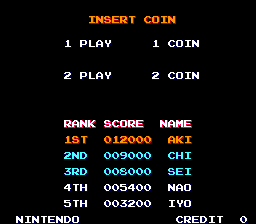
\includegraphics[width=0.25\textwidth]{img/highscore}};
\end{tikzpicture}
\end{Slide}

\begin{Slide}{Algoritmexempel: PRODUKTEN AV $n$ TAL}
\end{Slide}


\Subsection{Funktioner och procedurer skapar struktur}

\begin{Slide}{Block}\SlideFontSmall
Kapslar in många satser.

Vad är ett block?
I Scala (till skillnad från många andra språk) har ett block har ett värde 

\end{Slide}

\begin{Slide}{Block kan ha lokala variabler}\SlideFontSmall
Synlighetsregler etc
\end{Slide}


\begin{Slide}{Funktioner}\SlideFontSmall
\end{Slide}

\begin{Slide}{Parameter och argument}\SlideFontSmall
\end{Slide}

\begin{Slide}{Procedurer}\SlideFontSmall
\begin{itemize}
\item En \Emph{procedur} är en funktion som \Alert{gör} något intressant, men som \Alert{inte} lämnar något intressant returvärde.
\item Exempel på befintlig procedur: \code{println("hej")}
\item Du \Emph{deklarerar egna procedurer} genom att ange \texttt{\Alert{Unit}} som returvärdestyp. Då ges värdet \texttt{\Alert{()}} som betyder ''inget''.
\end{itemize}
\begin{REPL}
scala> def hej(x: String): Unit = println(s"Hej på dej $x!")
hej: (x: String)Unit

scala> hej("Herr Gurka")
Hej på dej Herr Gurka!

scala> val x = hej("Fru Tomat")
Hej på dej Fru Tomat!
x: Unit = ()
\end{REPL}
\begin{itemize}
\item Det som \Alert{görs} kallas (sido)\Emph{effekt}. Ovan är utskriften själva effekten.
\item Funktioner kan också ha sidoeffekter. De kallas då \Alert{oäkta} funktioner.
\end{itemize}
\end{Slide}

\begin{Slide}{Ingenting är faktiskt någonting i Scala}
I många språk (Java, C, C) är funktioner som saknar värden speciella. I Java finns nyckelordet  \jcode{void} men inte i Scala. I Scala är procedurer inte speciell efter som de faktisk returnerar ett värde som representerar ingenting, nämligen () som är av typen Unit. På så sätt blir procedurer inget undantag utan följer vanliga regler för syntax och semantik som för alla andra funktioner.

\url{https://en.wikipedia.org/wiki/Void_type}

\url{https://en.wikipedia.org/wiki/Unit_type}
\end{Slide}

\begin{Slide}{Abstraktion: Problemlösning genom nedbrytning i enkla funktioner och procedurer som kombineras}\SlideFontSmall
\begin{itemize}
\item En av de allra viktigaste principerna inom programmering är \Emph{funktionell nedbrytning} där  \Emph{underprogram} i form av funktioner och procedurer skapas för att bli byggstenar som kombineras till mer avancerade funktioner och procedurer.

\item Genom de namn som definieras skapas \Emph{återanvändbara abstraktioner} som kapslar in det funktionen gör. 

\item Problemet blir med bra byggblock lättare att lösa.

\item Abstraktioner som beräknar eller gör \Emph{en enda, väldefinierad sak} är enklare att använda, jämfört med de som gör många, helt olika saker.

\item Abstraktioner med \Emph{välgenomtänkta namn} är enklare att använda, jämfört med kryptiska eller missvisande namn.
\end{itemize}

\end{Slide}

\begin{Slide}{Exempel på funktionell nedbrytning}
$<<$kvadrat, stapel, rutnät i kojo$>>$ 
\end{Slide}


\begin{Slide}{Paket}
$<<$paket skapar katalogstruktur för kodfiler$>>$ 
\end{Slide}

\begin{Slide}{Jar-filer}
$<<$liknar zip-filer; packar ihop bytekod i en enda fil för enkel distribution$>>$ 
\end{Slide}

\subsection{Att göra denna vecka}


%%%
\frame{\frametitle{Att göra i Vecka \vecka: Förstå grundläggande kodstrukturer}
\begin{enumerate}
\item Laborationer är \Alert{obligatoriska}.\\ Ev. sjukdom måste anmälas \Alert{före} till kursansvarig!
\item Gör övning \texttt{programs}
\item OBS! Ingen lab denna vecka w02. Använd tiden att komma ikapp om du ligger efter!
\item Träffas i samarbetsgrupper och hjälp varandra att förstå.
\item Om ni inte redan gjort det: Gör klart \href{https://github.com/bjornregnell/lth-eda016-2015/tree/master/assignments}{samarbetskontrakt} och visa för handledare på resurstid.
\item \Alert{Koda på resurstiderna} och få hjälp och tips! 
\end{enumerate}
}








